\documentclass{article}

% if you need to pass options to natbib, use, e.g.:
\PassOptionsToPackage{numbers}{natbib}
\bibliographystyle{plainnat}
% before loading neurips_2020

% ready for submission
% use [final] or [preprint] for their associated versions
\usepackage[final]{neurips_2020}
\usepackage[nottoc,numbib]{tocbibind}

\usepackage{graphicx}       % include images/graphs
\usepackage[utf8]{inputenc} % allow utf-8 input
\usepackage[T1]{fontenc}    % use 8-bit T1 fonts
\usepackage{hyperref}       % hyperlinks
\usepackage{url}            % simple URL typesetting
\usepackage{booktabs}       % professional-quality tables
\usepackage{amsfonts}       % blackboard math symbols
\usepackage{nicefrac}       % compact symbols for 1/2, etc.
\usepackage{microtype}      % microtypography

\title{Room Classification from Connected Floor Plan Graphs}
\author{
Nicholas DeGroot \\
DSC 180A: Data Science Capstone \\
University of California San Diego\\
La Jolla, CA 92122 \\
\texttt{ndegroot@ucsd.edu}
}

\begin{document}

\maketitle

\begin{abstract}

    Recent work in computer vision has explored using machine learning to digitize the floor plan: the architectural diagrams home builders use when constructing a new home. Most work has been focused in "raster-to-vector" approaches, which attempt to turn raster images of the floor plan into a set of vectors describing a wall, window, or other 2D object. While post-processing has shown some success in associating detected rooms with their purpose, these approaches largely rely on supplementary information such as text descriptions and icon detection. We explore whether the spatial information of detected rooms is sufficient to determine its purpose. In particular, we show that a graphical encoding of room adjacencies contains enough information alone to achieve results far better then chance.
    
\end{abstract}

\section{Introduction}

Home builders and architects use floor plans everyday to coordinate construction efforts on complex projects. These documents detail exactly where every wall, window, and door is located, as well as the purpose of each room. Historically, they are shared through raster formats in printed documents or their modern PDF equivalent. While these formats are convenient for sharing, they are not easily machine-readable. In recent years, computer vision has been used to digitize these plans, turning them into a set of vectors describing the location of each wall, window, and door. This process is known as "raster-to-vector" conversion, and was first popularized for use with floor plans by \citet{rastertovec2017}. These digitized floor plans can then be used for a variety of downstream applications, such as higher fidelity collaboration, construction cost estimation, and 3D model generation.

While raster-to-vector approaches have shown great success, they are not without their limitations. Most approaches rely on supplementary information such as text descriptions and icon detection to associate detected rooms with their purpose - information that isn't available on other types of floor plans. For example, LiDAR sensors in modern iPhones have been able to generate a 3D floor plan by detecting room dimensions and locations through RoomPlan, but don't embed any textual information about the room purpose \cite{appleroomplan}.

Our approach echos that of \citet{floorgraphs2021}, which relied only on the spatial information of detected rooms to determine their purpose. Specifically, we encode the spatial information of each room in an adjacency graph, with nodes describing rooms and edges describing adjacent rooms. We examine the performance of a variety of graph neural networks (GNNs) on this task, as well as how they compare to their traditional multi-layer perceptron counterparts. We differ from \citet{floorgraphs2021} in that we use a more detailed but smaller dataset in Cubicasa5k \cite{cubicasa5k}. This allows us to explore whether the models can generalize to more specific floor plans, allowing us to classify up to 35 "top-level" room categories and 69 "sub-level" room categories. Our experiments show that a purely graphical approach to floor plan classification is capable of promising results.

\section{Methods}

\subsection{Data Cleaning \& Preprocessing}
We start with the SVG-labeled floor plans from Cubicasa5k \cite{cubicasa5k}. Each SVG describes a particular home, with each room labeled and bounded by a polygon. This is easily extracted via BeautifulSoup4 with the \verb|lxml| parser. From there, we extract the following metadata:

\begin{enumerate}
    \item \textbf{Room Name}: The name of the room, e.g. "Bedroom", "Attic", etc.
    \item \textbf{Polygon}: The polygon describing the room's boundary. This is modeled using Shapely.
\end{enumerate}

We further calculate the following attributes for each room:

\begin{enumerate}
    \item \textbf{Room Category}: The generic category of the room. Included categories:
          \begin{itemize}
              \item Corridor
              \item Storage
              \item Dining
              \item Room
              \item Kitchen
              \item Bedroom
              \item LivingRoom
              \item Bath
              \item Outdoor
              \item Garage
          \end{itemize}
    \item \textbf{Width}: The maximum width of the room polygon, in pixels.
    \item \textbf{Height}: The maximum height of the room polygon, in pixels.
    \item \textbf{Area}: The area of the room polygon, in pixels.
\end{enumerate}

The distribution of room category can be found in Figure \ref{fig:cat-dist}. The distribution of room width/height can be found in Figure \ref{fig:dim-dist}

\begin{figure}
    \centering
    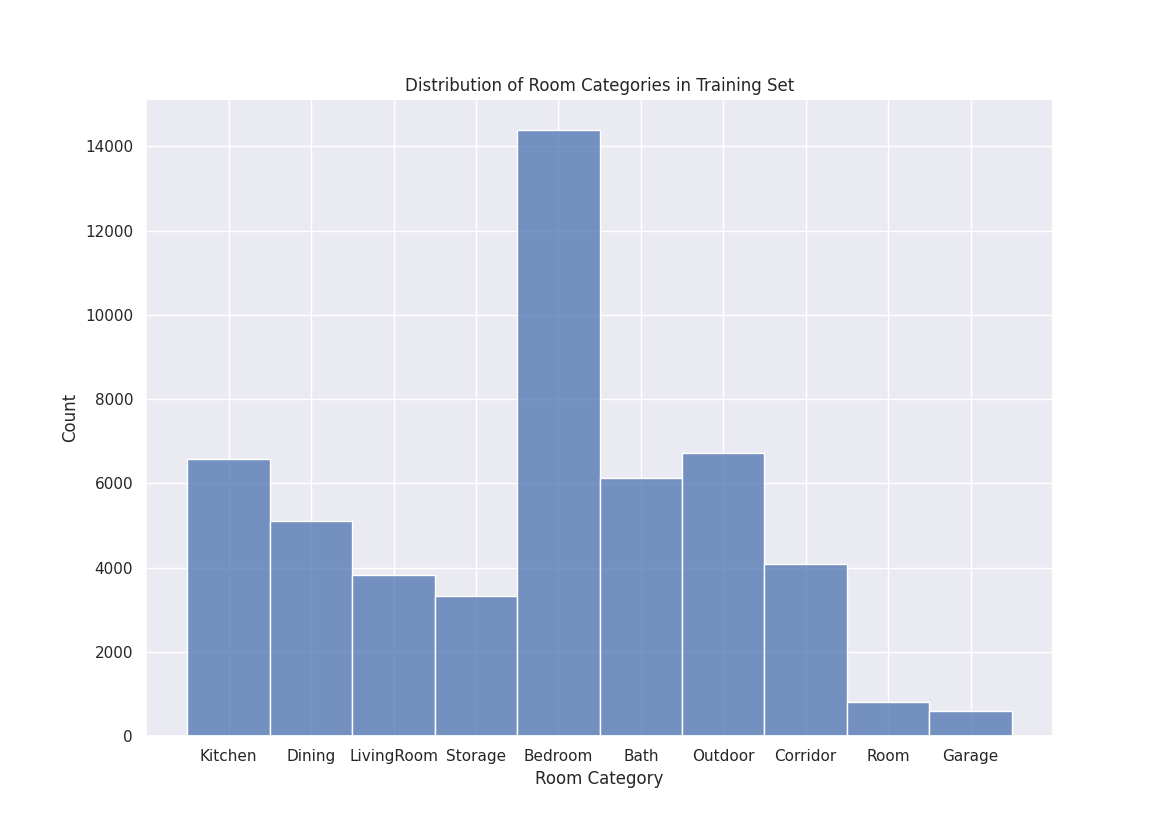
\includegraphics[width=.9\textwidth]{figures/cat-dist.png}
    \caption{Distribution of room categories in the training dataset.}
    \label{fig:cat-dist}
\end{figure}

\begin{figure}
    \centering
    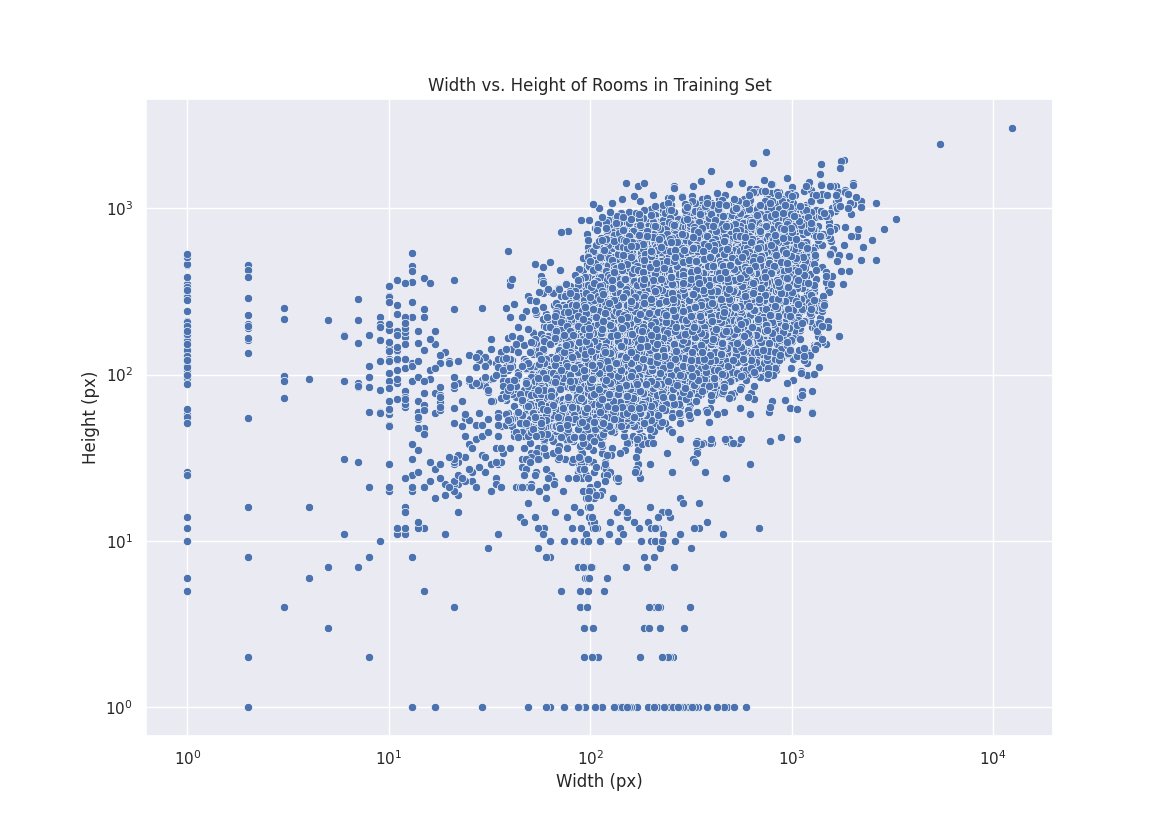
\includegraphics[width=.9\textwidth]{figures/dim-dist.png}
    \caption{Distribution of width/height in the training dataset.}
    \label{fig:dim-dist}
\end{figure}

For our last room-level attribute, we parse out all doors in the document using a similar method to rooms. We then buffer or extend each room's polygon by a small percentage, and check if the door polygon is contained within the room. If so, we add the door to the room's list of doors, and add the total number to each room.

For our graph-level attributes, we calculate all room adjacencies as edges. We do so much the same as we did for doors, but instead of checking if a door is contained within a room, we check if two rooms are adjacent. We define two rooms as adjacent if their buffered polygons intersect, or if one polygon is contained within the other.

Finally, we format the graph into a PyTorch Geometric Data object, which is the common language that all of our models speak. We use the width, height, area, and number of doors as our node attributes, and the adjacency as our edge attributes. Since this whole process can take awhile, we preprocess the entire dataset and save it to disk. This allows us to quickly load the data when training. The end result is approximately 40MB of compressed tensor data.

\subsection{Modeling}

We model the data using a variety of neural networks. We start with a simple baseline model: a simple feed-forward neural network. We then explore a variety of graph neural networks, including GraphSAGE \cite{graphsage}, Graph Convolutional Networks (GCN) \cite{gcn}, Graph Attention Networks (GAT) \cite{gat}, and Topology Adaptive Graph Convolutional Networks (TAGCN) \cite{tagcn}.

For each model, we use the Pytorch Geometric library \cite{pytorch_geometric} to implement a node-level classifier model that attempts to predict the room category. A hyperparameter determines how many layers of the associated model are used. After each layer, the outputs are ReLU activated and passed through. The model ends with a final linear classifier layer, which outputs the probability of a node belonging to a particular room category.

We use the Adam optimizer with a learning rate of 0.004 and a exponential rate scheduler with a gamma of 0.8. A batch size of 128 is used across 100 epochs. Cross entropy loss is used as our loss function. After competition, we save the best model by validation accuracy (per epoch) to disk.

All models were trained on an NVIDIA GeForce RTX 3080 GPU.


\section{Results}

To compare our models, we use the pre-portioned test dataset from Cubicasa5k and evaluate the models on the top-level room categories. Figure \ref{fig:accuracy} shows the accuracy of each model on the test set by number of hidden layers. The best seen combination came from the 10-layer GraphSAGE model, with an accuracy of 37.78\%. Even when restricted to 2 or 5 layers, the GraphSAGE model preformed best with accuracies of 30.27\% and 31.10\% respectively. The top reported accuracy for each model can be found in Table \ref{tab:results}.

\begin{figure}
    \centering
    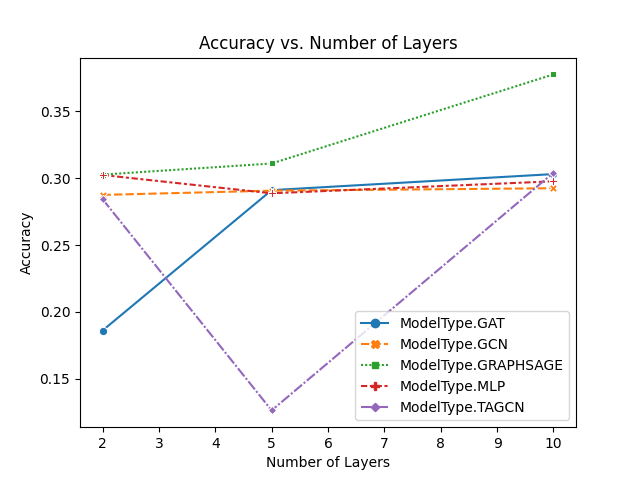
\includegraphics[width=.75\textwidth]{figures/acc-layers.png}
    \caption{Accuracy of each model on the test set.}
    \label{fig:accuracy}
\end{figure}

\begin{figure}
    \centering
    \begin{tabular}{lrr}
        \toprule
        Model Type & Accuracy & \# Layers \\
        \midrule
        GAT        & 0.303109 & 10        \\
        GCN        & 0.292511 & 10        \\
        GraphSAGE  & 0.377710 & 10        \\
        MLP        & 0.302429 & 2         \\
        TAGCN      & 0.304149 & 10        \\
        \bottomrule
    \end{tabular}
    \caption{Top accuracy for each model type.}
    \label{tab:results}
\end{figure}


\section{Discussion}

These results were surprising to us, as the original paper this study was based on reported much higher accuracies for nearly all models. While our models were barely able to scratch 40\% accuracy, \citet{floorgraphs2021} reported accuracies of 50\% and above, with the best models approaching 82\%. We believe that much of this is due to the difference in dataset. The dataset used in \citet{floorgraphs2021} was much larger, with a training set of over 20,000 floor plans, compared to our 4,194. Their dataset was also less diverse, with only 8 different room categories, compared to our 10. Finally, their methods were able to extract two additional attributes: whether a room is a parent or child room. We believe that these differences in dataset size and complexity are the primary reason for the discrepancy in results.

In addition, the ordering of model performance was different then reported by \citet{floorgraphs2021}. By 10-layers, a pretty clear model hierarchy of:

\begin{enumerate}
    \item TAGCN
    \item GraphSAGE
    \item MLP
    \item GCN
    \item GAT
\end{enumerate}

established itself. This is in contrast to our results, which have all models but GraphSAGE performing roughly the same. Most surprising is the TAGCN model, which we recorded as the worst performing with 5 layers (not doing much better then chance) as opposed to \citet{floorgraphs2021}'s best performing model. We can only speculate as to why this is, but believe it may be due to the differences in dataset discussed prior.

Regardless, we were still surprised at how well each model was at representing the data. Despite only having a grand total of 842 parameters (including a fully connected classifier!), the 2-layer GraphSAGE model was able to achieve an accuracy of 30.27\% - well above chance.

\section{Conclusion \& Future Work}

Overall, our experiments showed that graph neural networks are a promising approach to floor plan analysis. While we were unable to match the results of \citet{floorgraphs2021}, we were still able to achieve a respectable accuracy of 37.78\%. 

We believe that with a larger dataset and more complex models, we could achieve even better results. Given more time, we would like to explore a number of possible ways to better represent the data, including:

\begin{itemize}
    \item Encoding the shape of the room through a neural net
    \item Including recognized appliances
    \item Using different methods for calculating room adjacencies
    \item Experimenting with deeper models
\end{itemize}

Perhaps more practically, our methods could be combined with other methods of floor plan analysis, such as image recognition on the raster floor plan. Raster versions of floorplans are far more common then their graphical counterparts, and could be used to provide additional information about the floor plan. For example, the image could be used to identify appliances and extract the true dimensions of a room (instead of relative pixels). 

\bibliography{citations}

\end{document}
